\chapter{Non-dimensionalisation}\label{Non-dimensionalisation}
\begin{aquote}{Wild Thing. J. Bazell 2013.}
\textit{In metric, one milliliter of water occupies one cubic centimeter, weighs one gram, and requires one calorie of energy to heat up by one degree centigrade — which is 1 percent of the difference between its freezing point and its boiling point. An amount of hydrogen weighing the same amount has exactly one mole of atoms in it. Whereas in the [imperial] system, the answer to ``How much energy does it take to boil a room-temperature gallon of water?" is ``Go fuck yourself'', because you can't directly relate any of those quantities.}
\end{aquote}

Thus, far we have been fairly lax about defining the quantities we have actually been measuring. Further, once we have specified what the quantity actually is, what units are we using to measure the quantity. For example, if we are measuring distance are we doing it in mm, miles or light-years? Equally, is time measured in seconds, minutes or hours? Finally, constitutive laws often introduce parameters that are not quantified accurately, or alternatively, we may be interested in understanding how a solution depends on a particular parameter as it is varied. 

The Law of Mass Action, in particular, could be thought to be a troublesome law as it introduces a rate parameter for each reaction equation that is considered. For example, if a system of ODEs is defined by a set of non-linear equations it is highly unlikely to be solvable in closed form. Thus, if there are a large number of parameters in the system, it becomes very difficult to predict how varying a single parameter (or group of parameters) will influence the solution.

However, we have already seen cases in which we do not need to consider parameters individually, as specific groups of the parameters are seen to act in the same way. For example, in the case of the spring pendulum (see \sect{Pendulums_section}), we saw that the frequency of oscillation depended on $\sqrt{k/m}$. Thus, stiffening the spring (increasing $k$) has the same effect on the solution as decreasing the mass (decreasing $m$), \ie they both increase the frequency of the oscillations. Equally, in the example of a zombie infection (see example \ref{Zombies}), the parameters of interest were not $a$, $b$ or $c$, but rather $\alpha=b+c$ and $\beta=c-a$.

In this chapter we introduce a technique, called non-dimensionalisation, that will benefit us in two ways. Firstly, it allow us to brush away worries about dealing with units and, secondly, it will allow us to reduce the number of effective parameters in our system. Specifically, we will be able to define parameter groupings that will influence the final result in the same way.

\section{The central idea}
To non-dimensionalise a system of equations, we have the following rules:
\begin{enumerate}
\item Identify all the variables;
\item Replace each variable with a quantity scaled relative to a characteristic unit of measure (to be determined);
\item Choose the definition of the characteristic unit for each variable;\label{Choose}
\item Rewrite the system of equations in terms of the new dimensionless quantities.
\end{enumerate}
We note three particular points about these rules. Firstly, the theory behind non-dimensionalisation is straight forward. Namely, we substitute scaled variables into an equation system and massage the equations until we have rearranged the system to produce the desired outcome. However, in practice the difficulty of the technique lies in the algebraic manipulation; it is very easy for the terms to become lost during the manipulation. Thus, care must be taken during the algebraic manipulation stage.

Secondly, you will notice the word `choose' in point \ref{Choose}. This means that it possible to construct many different non-dimensionalised systems from the same system of equations, \ie non-dimensionalisation is non-unique. We usually choose the characteristic unit of each variable to either emphasise one of the terms in a system or to remove as many parameters as possible.

Finally, this technique is hard to demonstrate in generality. It is much better to consider a number of system and see how the technique works in action. Thus, what follows will be a select number of examples, which along with your problem sheets should give you a good basis in the theory. However, do not think that these are all the examples you could face.

It should be noted that there is little consistency in nomenclature across book when considering the separation of variables into their dimensional and non-dimensional components. Thus, always be clear in your definitions.

\subsection{Examples of non-dimensionalisation through substitution of variables}\label{Examples of non-dimensionalisation through substitution of variables}
\begin{example}[frametitle=Substituting variables]
\begin{itemize}
\item Consider the equation for exponential growth,
\bb
\dot{u}=ru, \quad u(0)=u_0.\label{Non-dim_1}
\ee
\COL{The variables in \eqn{Non-dim_1} are $u$ and $t$. We rewrite them as $u=[u]u'$ and $t=[t]t'$, where $[u]$ and $[t]$ are the dimensional scales and $u'$ and $t'$ are the non-dimensional variables. We are free to define the values of $[u]$ and $[t]$ as we please. It is our job to choose appropriate definitions that simplify \eqn{Non-dim_1}. Critically, although we are free to choose the value of $[u]$ and $[t]$ the values must have consistent units. Namely, $[t]$ must have units of time and $[u]$ must have units of density.

We substitute the expanded variables into \eqn{Non-dim_1} and rearrange to produce
\bb
\frac{\rd u'}{\rd t'}=[t]ru', \quad u(0)=\frac{u_0}{[u]}.\nonumber
\ee
Hence, we see that if we choose $[t]=1/r$ and $[u]=u_0$ then \eqn{Non-dim_1} simplifies to
\bb
\dot{u}=u, \quad u(0)=1,\nonumber
\ee
where we note that we have dropped the prime symbols, $'$, for notational convenience.

For mathematicians dropping primes is often done as the last step because we infrequently care about the actual values of the variables, rather we study the dynamics available in the equation. However, in any specific application we should be careful to remember that the variables we are dealing with are non-dimensional and that the solution is not complete until we `re-dimensionalise' the variables.}

\COL{In this example we see that the values of $r$ and $u_0$ in \eqn{Non-dim_1} do not influence the dynamics of the simulation. Specifically, they only scale the time and initial condition.

Although this was a fairly trivial example, a good way to check consistency of the answer at the end of the manipulation is to check that all of the dimensions agree. As mentioned $[t]$ should have units of time and $[u]$ should have units of density. We return to \eqn{Non-dim_1} and consider the dimensions of each component.

For example, $\dot{u}=\rd u/ \rd t$ has units of density/time. By equality, $ru$ must have units of density/time since $u$ has units of density then $r$ must have units of 1/time. Thus, 
\bb
\textrm{dim}([t])=\textrm{dim}(1/r)=\textrm{time}.\nonumber
\ee
Equally, $[u]=u_0$ can trivially be seen to have the correct units of density.}

\item Consider the equation for logistic growth,
\bb
\dot{u}=ru\l 1-\frac{u}{K} \r, \quad u(0)=u_0.\label{Non-dim_2}
\ee
\COL{Again, $u=[u]u'$ and $t= [t]t'$ can be substituted into \eqn{Non-dim_2} to produce
\bb
\frac{\rd u'}{\rd t'}=[t]ru'\l 1-\frac{[u]}{K}u'\r,\quad u'(0)=\frac{u_0}{[u]},\nonumber
\ee
from which we see that it would be wise to once again take $[t]=1/r$. Beyond this we see that we have a choice. Should we take $[u]=K$, or $[u]=u_0$? Both are valid non-dimensionalisations and either maybe be appropriate depending on the context of the problem. 

Here, we are going to take $[u]=K$ as we are interested in the dynamics of the system, rather than the initial condition. Thus, after dropping primes we see that we can non-dimensionalise \eqn{Non-dim_2} to 
\bb
\frac{\rd u}{\rd t}=u\l 1-u\r,\quad u(0)=U_0,\nonumber
\ee
where $U_0=u_0/[u]=u_0/K$.

In this case the non-dimensionalisation demonstrates that the only parameter that the solution depends on is the initial conditions. Changing $r$ does not change the dynamics of the system, it only changes the time scale, since $r=1/[t]$. Equally, changing $K$ simply scales the size of the solution, as $u=Ku'$.}

\item Consider the following equations (the Schnakenberg kinetics)
\begin{align}
&\dot{u}=k_1-k_2u+k_3u^2v, \quad u(0)=u_0,\label{Non-dim_31}\\
&\dot{v}=k_4-k_3u^2v, \quad v(0)=v_0.\label{Non-dim_32}
\end{align}
\COL{This time we use the scales $u=[u]u'$, $v=[v]v'$, $t=[t]t'$ to derive
\begin{align}
&\frac{\rd u'}{\rd t'}=\frac{[t]k_1}{[u]}-[t]k_2u'+[t]k_3[u][v]u'^2v', \quad u'(0)=\frac{u_0}{[u]},\nonumber\\
&\frac{\rd v'}{\rd t'}=\frac{[t]k_4}{[v]}-[t]k_3[u]^2u'^2v', \quad v'(0)=\frac{v_0}{[v]}.\nonumber
\end{align}}\COL{
Lots of potential choices for scale balances; how do we choose? In an exam you will be given the form of an equation to produce and your task will be to derive the corresponding scales. For example, suppose we wanted to convert \eqns{Non-dim_31}{Non-dim_32} into
\begin{align}
&\frac{\rd u'}{\rd t'}=\alpha-u'+u'^2v', \quad u'(0)=u'_0\nonumber\\
&\frac{\rd v'}{\rd t'}=\beta-u'^2v', \quad v'(0)=v'_0,\nonumber
\end{align}
then we know that we would have to set
\bb
1=[t]k_3[u][v]=[t]k_2=[t]k_3[u]^2.\nonumber
\ee
Thus,
\begin{align}
&[t]=\frac{1}{k_2},\nonumber\\
&[u]=\sqrt{\frac{1}{[t]k_3}}=\sqrt{\frac{k_2}{k_3}},\nonumber\\
&[v]=[u]=\sqrt{\frac{k_2}{k_3}},\nonumber
\end{align}
which means that
\begin{align}
\alpha=\frac{[t]k_1}{[u]}=\frac{k_1}{k_2}\sqrt{\frac{k_3}{k_2}},\nonumber\\
\beta=\frac{[t]k_4}{[v]}=\frac{k_4}{k_2}\sqrt{\frac{k_3}{k_2}},\nonumber\\
u'_0=\frac{u_0}{[u]}=u_0\sqrt{\frac{k_3}{k_2}},\nonumber\\
v'_0=\frac{v_0}{[v]}=v_0\sqrt{\frac{k_3}{k_2}}.\nonumber
\end{align}

Finally, we check the consistency of the scales. From \eqns{Non-dim_31}{Non-dim_32} we infer that
\bb
\textrm{dim}(k_1)=\frac{\textrm{density}}{\textrm{time}}, \quad \textrm{dim}(k_2)=\frac{1}{\textrm{time}}, \quad \textrm{dim}(k_3)=\frac{1}{\textrm{density}^2\textrm{time}}, \quad \textrm{dim}(k_4)=\frac{\textrm{density}}{\textrm{time}}.\nonumber
\ee
Hence,
\bb
\textrm{dim}([u])=\sqrt{\frac{1/\textrm{time}}{1/(\textrm{density}^2\textrm{time})}}=\sqrt{\textrm{density}^2}=\textrm{density}.
\ee
The scales $[v]$ and $[t]$ can be checked similarly. We also need to ensure the the variables $\alpha, \beta, u'_0, v'_0$ are have no dimension. For example
\bb
\textrm{dim}(v'_0)=\textrm{density}\sqrt{\frac{1/(\textrm{density}^2\textrm{time})}{1/\textrm{time}}}=\textrm{density}\sqrt{\frac{1}{\textrm{density}^2}}=1.
\ee
The other variables can be checked similarly.}
\end{itemize}
\end{example}

\subsection{Examples of non-dimensionalisation through the arrow method}
The substitution method shown in \sect{Examples of non-dimensionalisation through substitution of variables} will always work supposing that the algebra is manipulated correctly. However, the method can be cumbersome and slow. Moreover, because it involves lots of algebraic manipulations there are many chances to make a mistake.

An alternative method rests on using arrows to identify the desired balances. This can be much quicker as the initial stages do not require laborious substitution. However, we have to be more careful because not all balances that we can `draw' using the arrows will be valid.

The idea behind the arrow method is that you draw arrows between the quantities that are going to `balance', which simply means they are going to have the same coefficient in the final non-dimensionalised form. The process is generally the same as the substitution method. However, we must remember that in order to specify the problem completely the number of valid arrow balances must equal the number of variables. For example, if a problem depends on $u$ and $t$ we would need two balances. Alternatively, if the problem depended on $u$, $v$, and $t$ we would need three valid balances.  This section is going to depend primarily on examples, again, and we will see an invalid balance at the end of the demonstrations.
\begin{example}[frametitle=Arrow method]\label{Arrow method}
\item Consider the following equation
\bb
  \tikzmark{a}\dot{u}=k_0+k_1\tikzmark{b}u+k_2\tikzmark{c}u^2, \quad u(0)=u_0.\label{Non-dim_4}
\tikz[overlay,remember picture]
{\draw[square arrow1] (a.south) to (b.south);}
\tikz[overlay,remember picture]
{\draw[square arrow1] (b.south) to (c.south);}
\ee
\COL{We have two variables, $u$ and $t$, and so we need two balances. Specifically, the arrows state that we want to balance the derivative, linear and quadratic terms,
\bb
\frac{[u]}{[t]}=k_1[u]=k_2[u]^2,\nonumber
\ee
from which it is simple to discover that
\bb
[t]=\frac{1}{k_1},\quad [u]=\frac{k_1}{k_2}.\nonumber
\ee
We still need to substitute the scales into the equations. Namely, $u=u'k_1/k_2$ and $t=t'/k_1$, but again the arrow method simplifies this task. Specifically, we know that, by design, the coefficient of the derivative, linear and quadratic term are going to be the same. Thus, we can divide through by one of them to speed up the derivation,
\bb
\frac{\rd u'}{\rd t'}=\frac{k_0}{k_1[u]}+u'+u'^2.\nonumber
\ee
Finally, redefining the last parameter as $\alpha=k_0/(k_1[u])=k_0k_2/(k_1^2)$ and the initial condition $u'(0)=k_2u_0/k_1=u'_0$, we can non-dimensionalise \eqn{Non-dim_4} to the final form of
\bb
\dot{u}=\alpha+u+u^2,\quad u(0)=u'_0,\label{Non-dim_5}
\ee
where we have dropped the primes from the variables for simplicity. Once again, we would have to ensure that $\alpha$ and $u'_0$ where non-dimensional and that $[u]$ and $[t]$ had the right dimensions, but this }\COL{is left as an exercise.
}\COL{
In this example we can illustrate the power of the non-dimensionalisation through the parameter groupings
\bb
\alpha=\frac{k_0k_2}{k_1^2},\quad u'_0=\frac{k_2u_0}{k_1}.\nonumber
\ee
Specifically, suppose we double each of the kinetic parameters \ie $k_0\mapsto 2k_0$, $k_1\mapsto 2k_1$ and $k_2\mapsto 2k_2$ then neither $\alpha$, nor $u'_0$ changes. This means that under this transformation the solution of \eqn{Non-dim_5} is exactly the same. But, how does this transformation of the original equations? Well, $[u]=k_1/k_2$ does not change, but $[t]=1/(2k_1)$ will be half its previous value. Hence, the solution to this `doubled-parameter' problem (call it $u_2(t)$) will reach the same solution values as the original problem, but in half the time \see{Non_dim_example},
\bb
u_2(t)=u\l\frac{t}{2}\r.\label{Non-dim_6}
\ee}

% we notice that if we double the value of $k_2$ and simultaneously half $k_0$ and $u_0$ then the values of $\alpha$ and $u'_0$ do not change, this means that the solution of \eqn{Non-dim_5} is the same under this transformation and, thus, so must the solutions of \eqn{Non-dim_4}.
\end{example}
\begin{figure}[!!!h!!!tb]
\centering
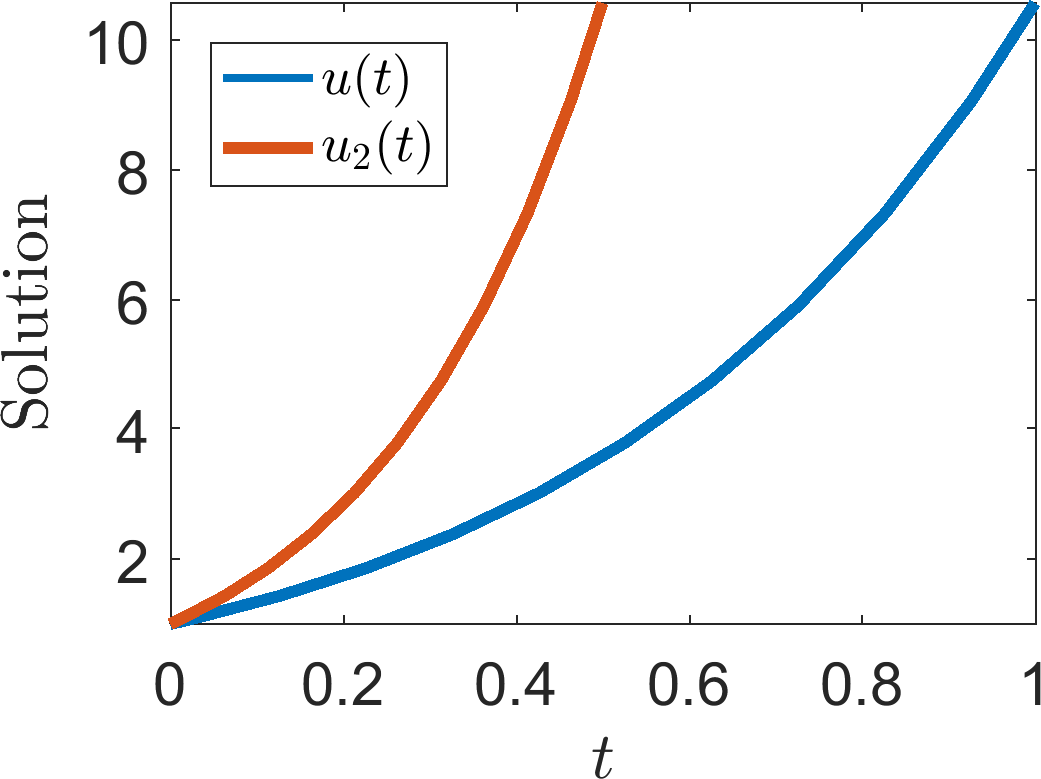
\includegraphics[width=\ttp]{../Pictures/Non_dim_example.png}
\caption{\label{Non_dim_example} Two simulations of \eqn{Non-dim_4} with parameter values $k_0=k_1=k_2=1$ (blue line, $u(t)$) and $k_0=k_1=k_2=2$ (red line, $u_2(t)$). Illustrating that the evolution of the red line is the same as the blue line, except that the red line evolution occurs twice as fast, as predicted by \eqn{Non-dim_6}.}
\end{figure}

\begin{example}[frametitle=Non-uniqueness]
 To illustrate the non-uniqueness of non-dimensionalisation we rerun example \ref{Arrow method} but this time we balance the time derivative, the constant term and the initial condition,
\bb
  \tikzmark{a}\dot{u}=k_0\tikzmark{b}+k_1u+k_2u^2, \quad u\tikzmark{c}(0)=u_0\tikzmark{d}.\label{Non-dim_7}
\tikz[overlay,remember picture]
{\draw[square arrow1] (a.south) to (b.south);}
\tikz[overlay,remember picture]
{\draw[square arrow1] (c.south) to (d.south);}
\ee
\COL{We quickly find that
\bb
\frac{[u]}{[t]}=k_0,\quad [u]=u_0,\nonumber
\ee
thus, $[t]=u_0/k_0$. We can divide the equation through by $k_0$, because we know that this is the }\COL{balance of the first two terms in \eqn{Non-dim_7}. Thus, we derive
\bb
\dot{u'}=1+\frac{k_1[u]}{k_0}u'+\frac{k_2[u]^2}{k_0}u'^2, \quad u'(0)=1,\nonumber
\ee
which would be rewritten as
\bb
\dot{u}=1+\beta u+\gamma u^2, \quad u(0)=1,\label{Non-dim_8}
\ee
where
\bb
\beta=\frac{k_1u_0}{k_0},\quad \gamma=\frac{k_2u_0^2}{k_0}.\nonumber
\ee}
\end{example}

Both forms of the non-dimensionalised equation, \eqref{Non-dim_5} and  \eqref{Non-dim_8}, are perfectly valid. The most useful form will depend on what factor dominates the equation. If $k_0$ is small and $k_1$ is big (relative to one another) then \eqn{Non-dim_5} would be more useful as $\alpha\approx0$ and we would be able to manipulate the equation to provide more information. Alternatively, if $k_0$ was big and $k_2$, or $k_1$, was small then, \eqn{Non-dim_8} would be more useful as we would, again, be able to remove one of the constants based on this assumption.

\begin{example}[frametitle=Failure]
As mentioned not all balances are valid, which is what we will be seen in this example. Consider the following ODE system
\begin{align}
  \tikzmark{a}\dot{u}=k_0\tikzmark{b}+k_1\tikzmark{c}u-k_2uv, \quad u(0)=u_0,\\
 \nonumber \\
    \tikzmark{e}\dot{v}=k_3\tikzmark{f}+k_4\tikzmark{g}v-k_2uv, \quad v(0)=v_0.
\tikz[overlay,remember picture]
{\draw[square arrow1] (a.south) to (b.south);}
\tikz[overlay,remember picture]
{\draw[square arrow1] (b.south) to (c.south);}
\tikz[overlay,remember picture]
{\draw[square arrow1] (e.south) to (g.south);}
\end{align}
\COL{There are three variables $u$, $v$ and $t$ and so we need three balances. The chosen balances are illustrated on the equations using arrows. Extracting information from the balances we find that
\bb
\frac{[u]}{[t]}=k_0=k_1[u], \quad \frac{[v]}{[t]}=k_4[v].
\ee
From this point we quickly discover that
\bb
[t]=\frac{1}{k_1} \textrm{ and } [t]=\frac{1}{k_4}.
\ee
Since, generally, $k_1\neq k_4$ we cannot satisfy both balances, thus, we must consider a different non-dimensionalisation.}

One possible valid non-dimensionalisation is
\begin{align}
  \tikzmark{a}\dot{u}=k_0\tikzmark{b}+k_1\tikzmark{c}u-k_2uv, \quad u(0)=u_0,\nonumber\\
 \nonumber \\
    \tikzmark{e}\dot{v}=k_3\tikzmark{f}+k_4\tikzmark{g}v-k_2uv, \quad v(0)=v_0.\nonumber
\tikz[overlay,remember picture]
{\draw[square arrow1] (a.south) to (b.south);}
\tikz[overlay,remember picture]
{\draw[square arrow1] (b.south) to (c.south);}
\tikz[overlay,remember picture]
{\draw[square arrow1] (e.south) to (f.south);}
\end{align}
See the board for details.
\end{example}

Although each case of non-dimensionalisation is different, the algorithm you should follow is the same in each case. The steps are:
\begin{enumerate}
\item write down the variables in the equations, this tells you how many balances you need;
\item specify balances and check that they are valid;
\item define non-dimensional scales that allow you to minimise the number of free parameters;
\item substitute the scales into the equations and collect together the remaining parameters into the smallest possible groups and give them a new variable name (DO NOT FORGET to do the same thing for the initial conditions. Everyone always forgets to do the initial conditions);
\item demonstrate that the scales you have derived have the correct dimension;
\item demonstrate that the new parameter groupings are dimensionless.
\end{enumerate}
Although we have not completed the last two points for every example, you will be expected to do every step in an exam.
%\begin{figure}[!!!h!!!tb]
%\centering
%\subfigure[\label{IC_0.1}]{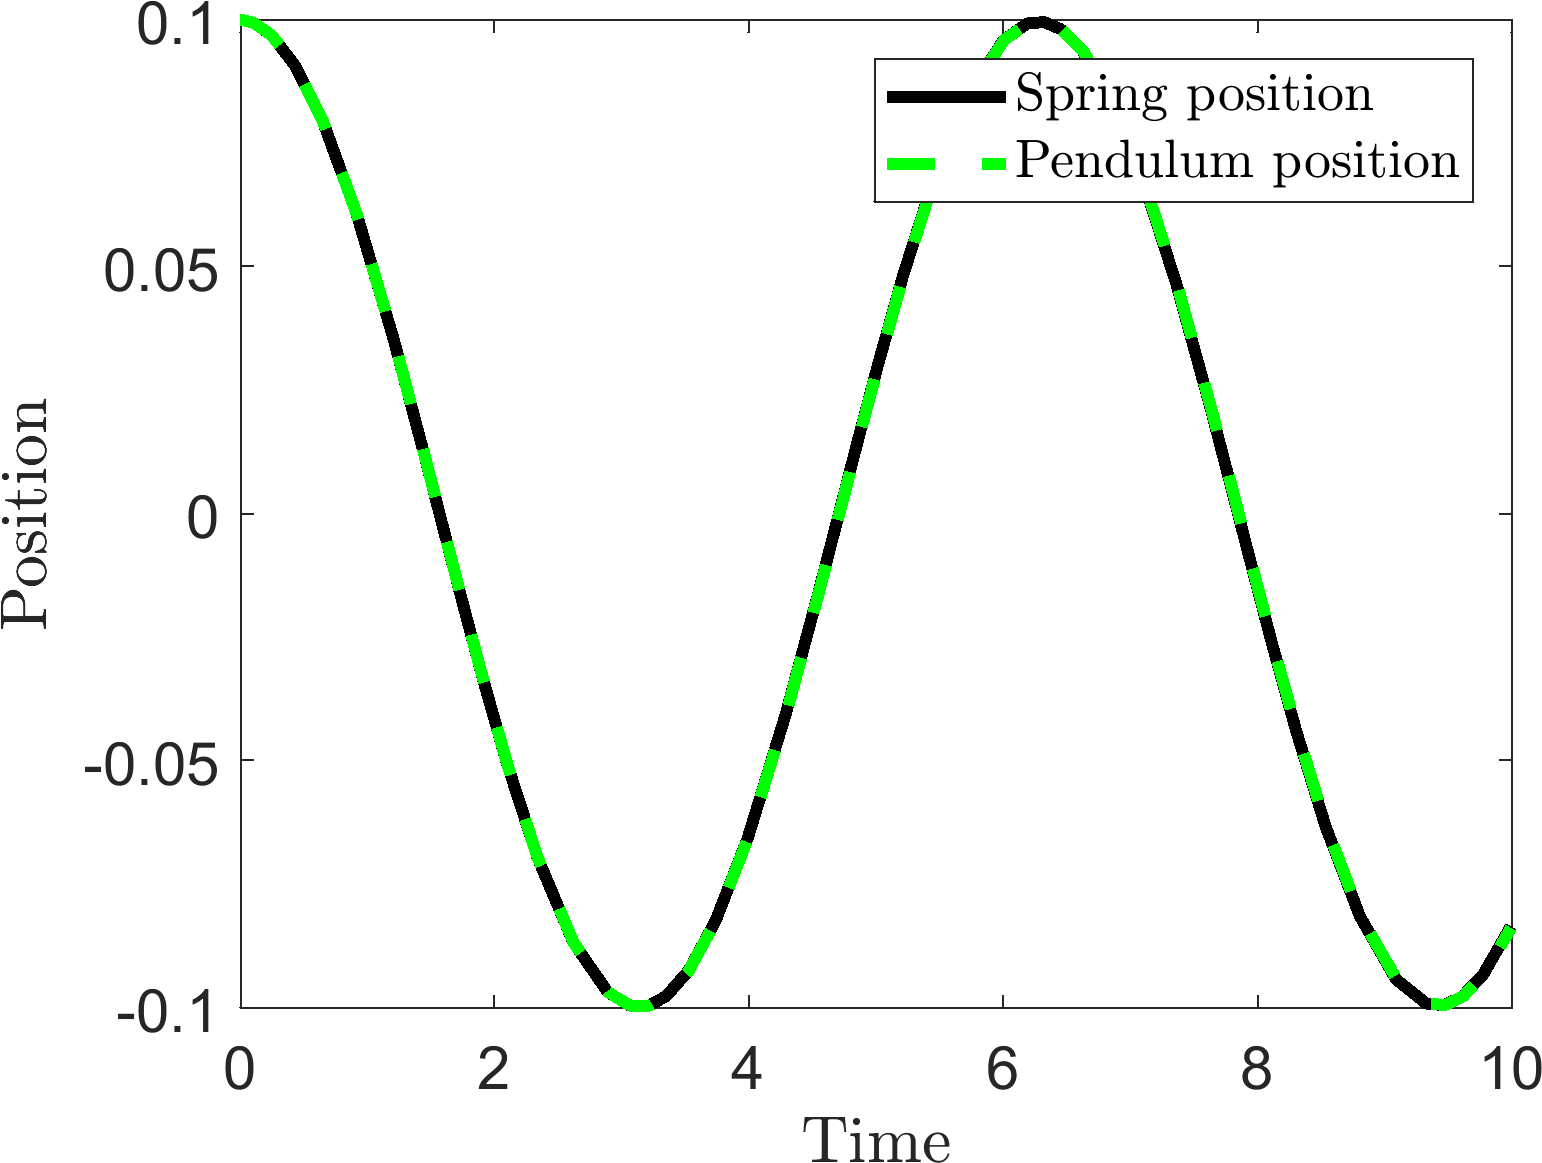
\includegraphics[width=\ttp]{../Pictures/Comparing_pendulums_IC_1.png}}
%\subfigure[\label{IC_1}]{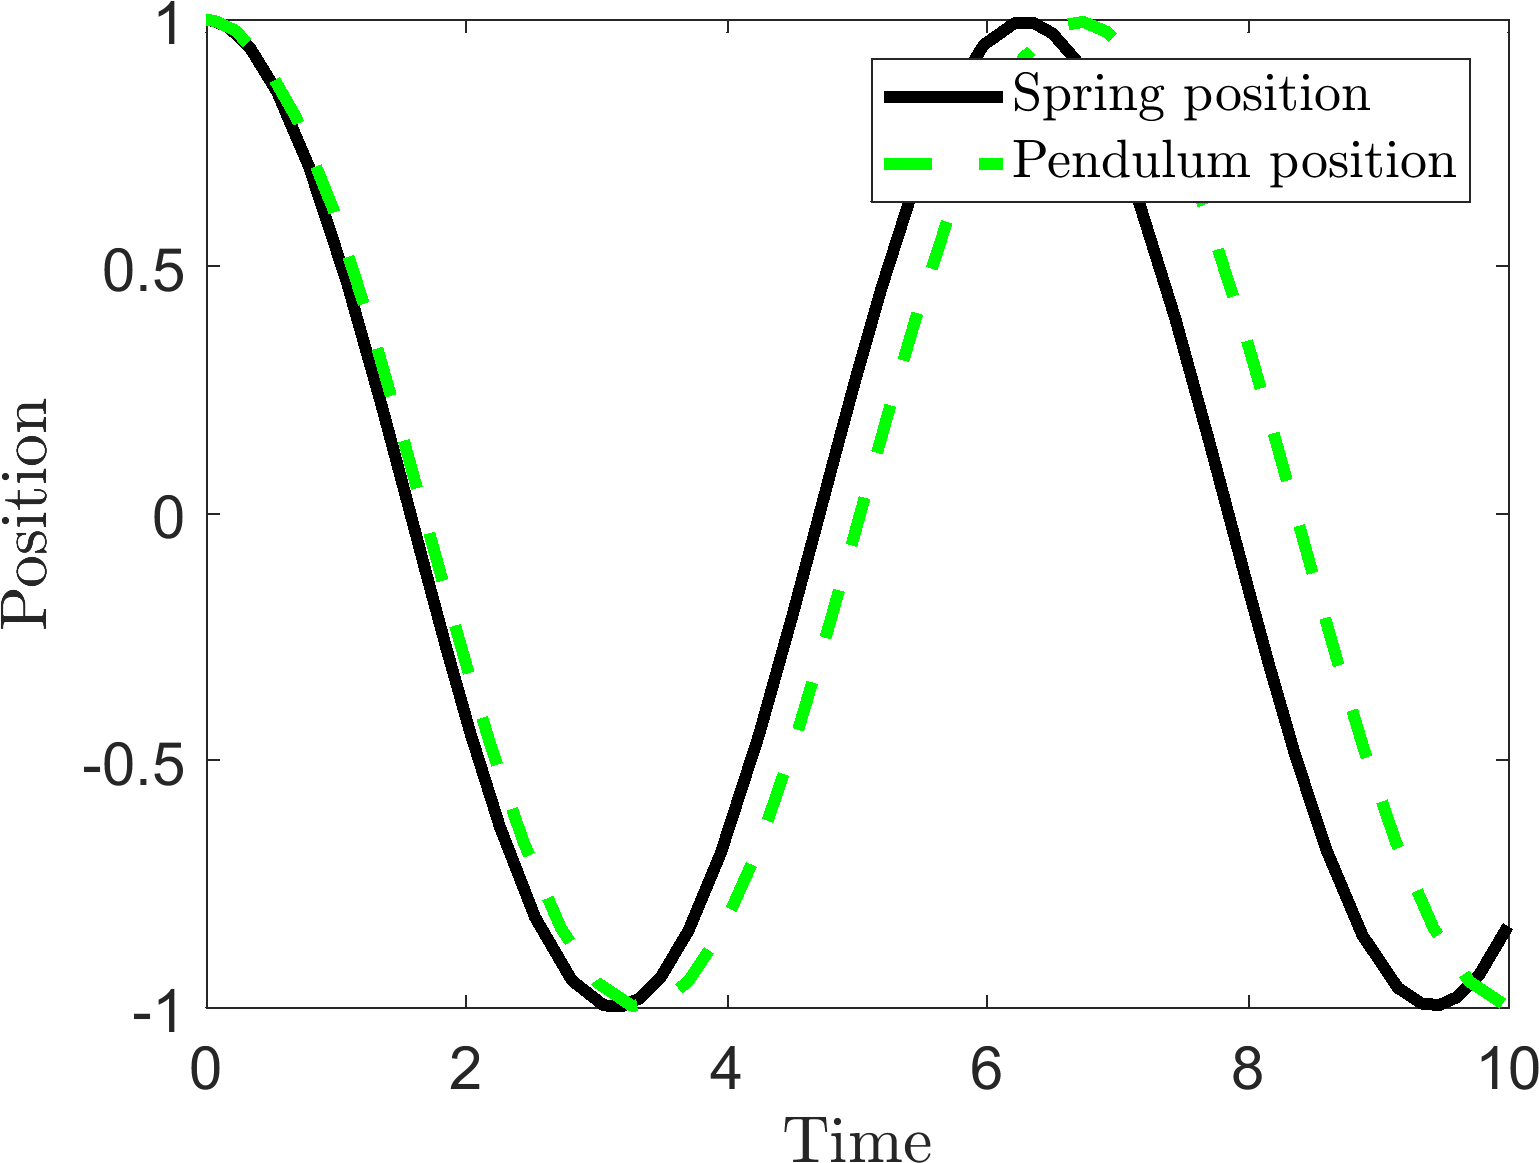
\includegraphics[width=\ttp]{../Pictures/Comparing_pendulums_IC_10.png}}
%\caption{\label{Different_ICs}Comparing \eqns{Spring_eqn}{Bob_eqn} with initial conditions (a) $y=0=\theta$ and (b) $y=1=\theta$. Parameter values $r=g=k=m=1$.}
%\end{figure}
%
%
%\begin{example}[frametitle=Zombies]\label{Zombies}
%Humans, $H$ and zombies, $Z$ interact through the following three interactions \see{Zombie_picture}]:
%\end{example}
%\begin{figure}[!!!h!!!tb]
%\centering
%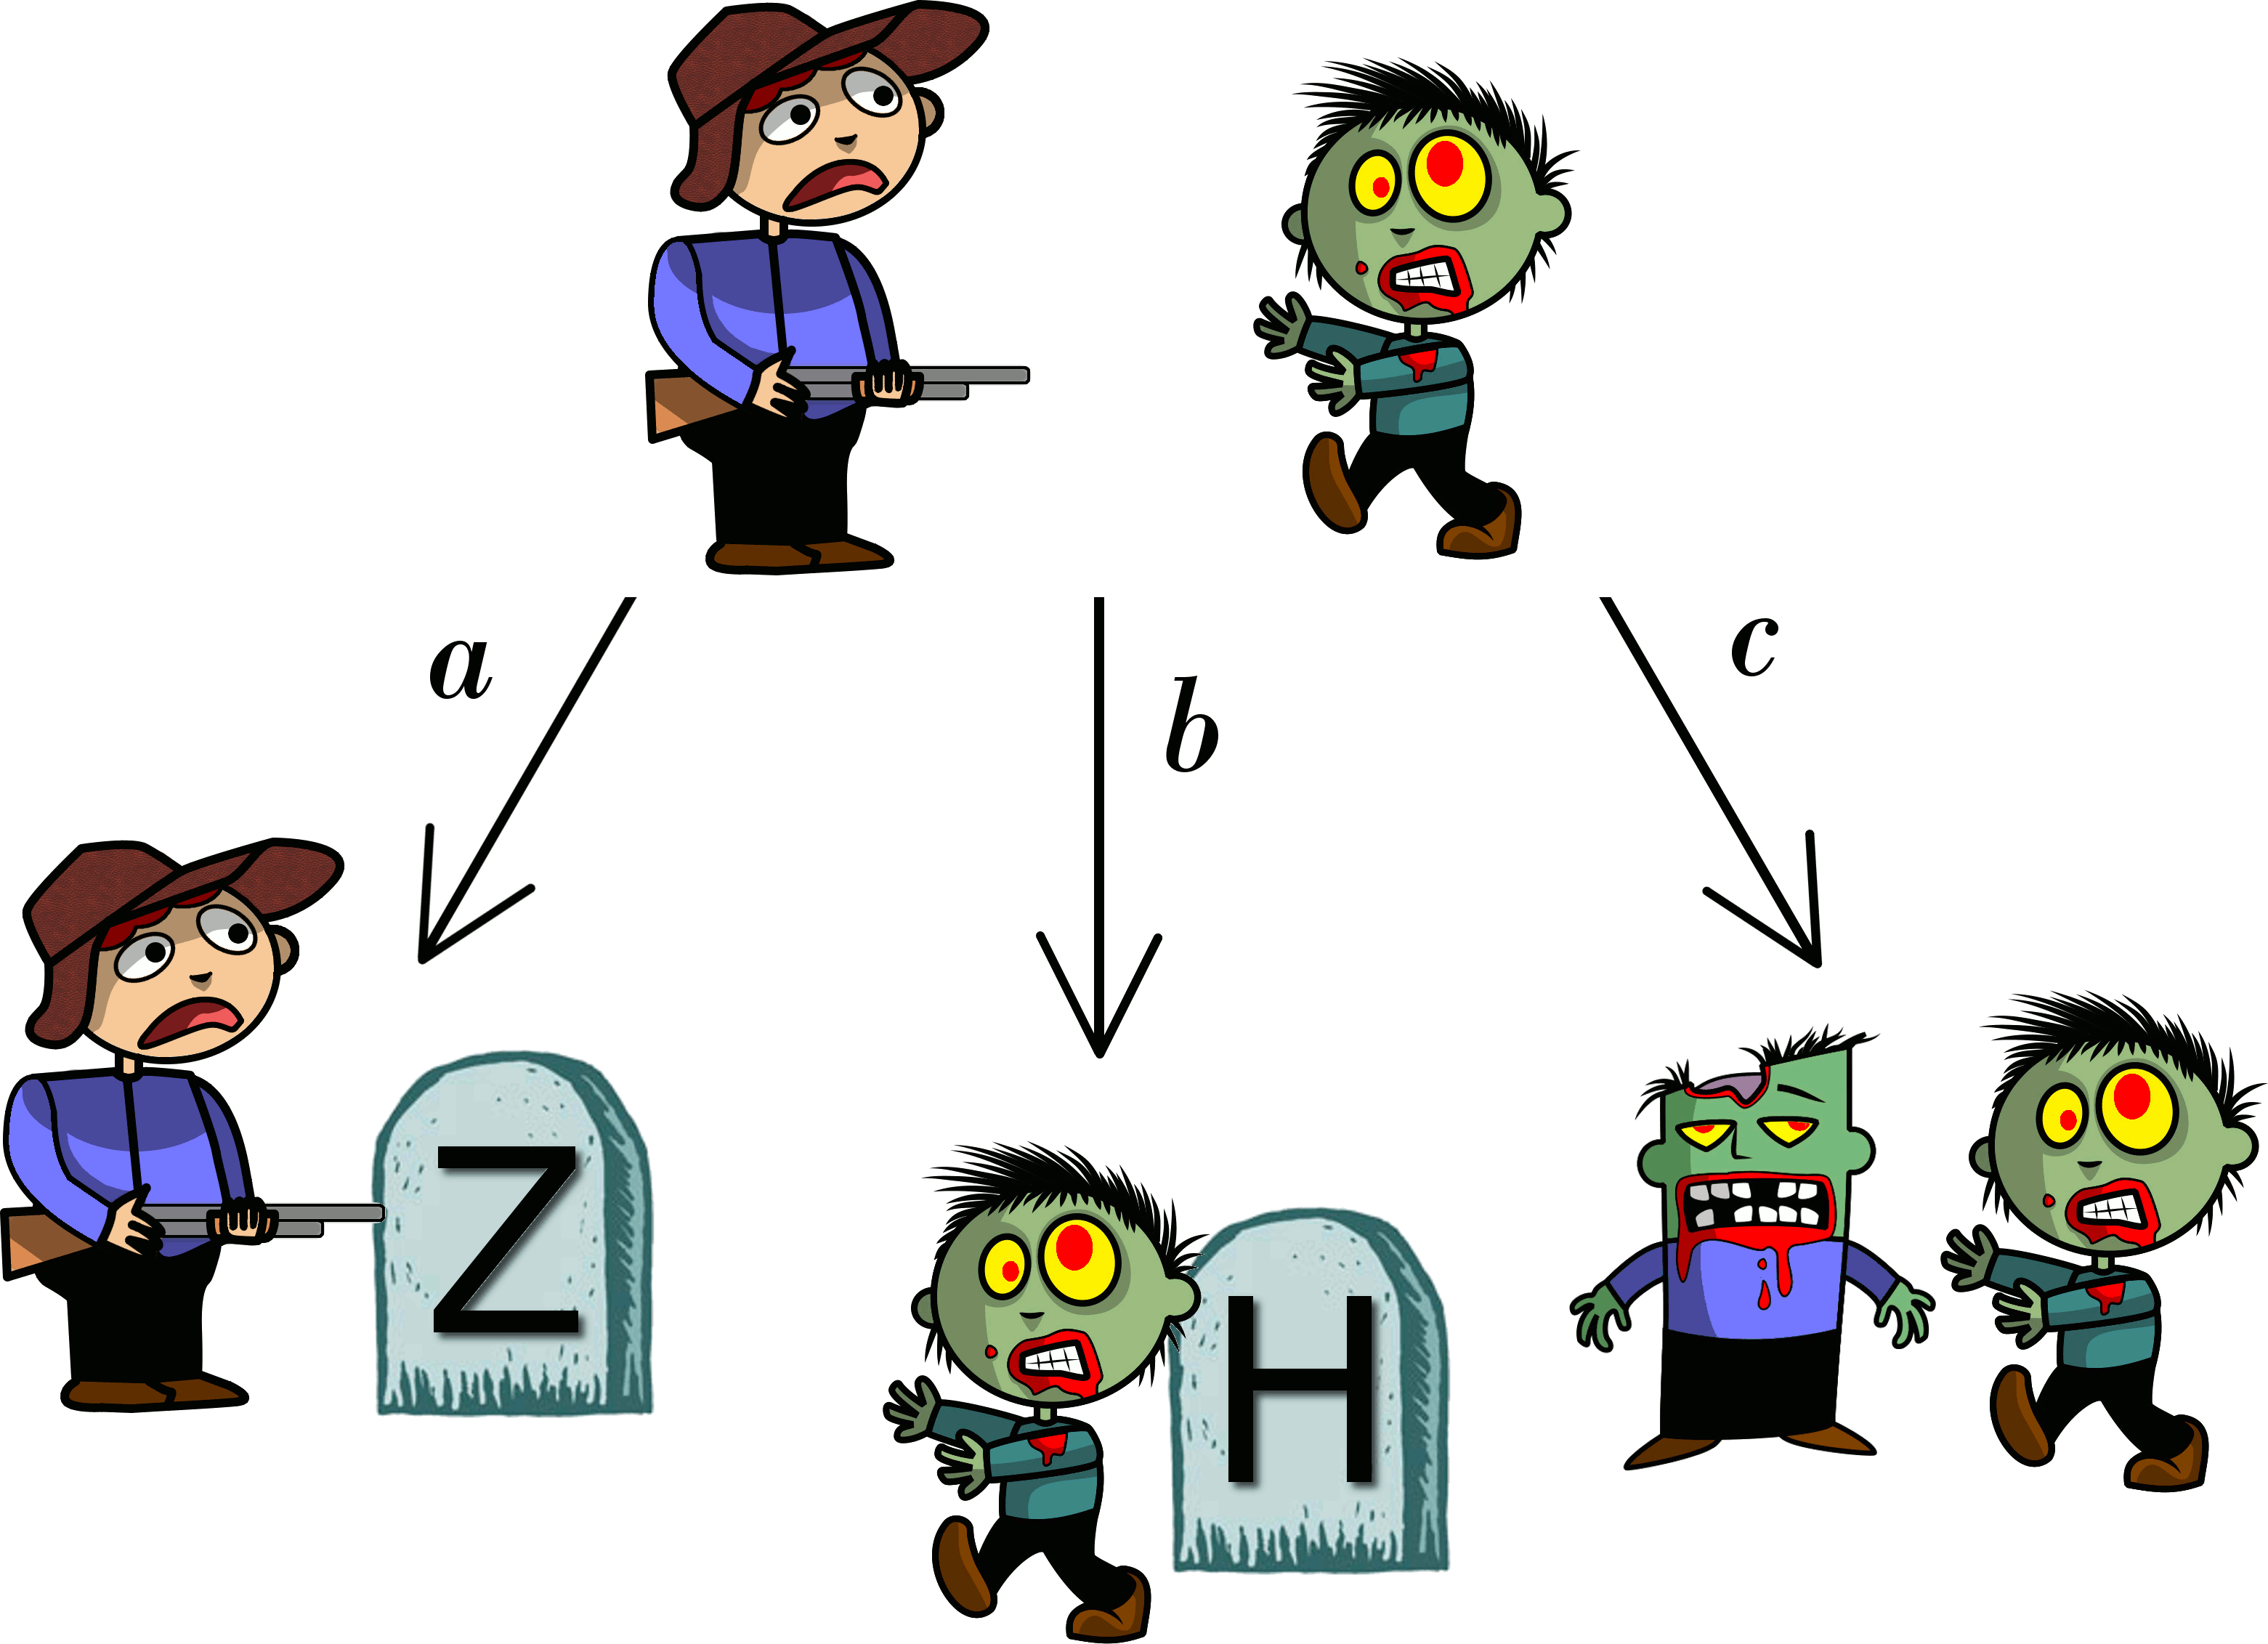
\includegraphics[width=\tp]{../Pictures/Zombies.png}
%\caption{\label{Zombie_picture} Possible outcomes of human-zombie interactions.}
%\end{figure}

\section{Check list}
By the end of this chapter you should be able to:
\begin{todolist}
\item non-dimensionalise a system of equations using direct substitution, or the arrow method;
\item demonstrate that the derived scales have the correct dimension;
\item demonstrate that remaining parameter groupings are non-dimensional;
\end{todolist}




